\documentclass[12pt,fleqn]{article}
\usepackage{amsfonts,amsthm,amsopn,amssymb,latexsym}
\usepackage{hyperref}
\usepackage{graphicx}
\usepackage[T1]{fontenc}
\usepackage[brazil]{babel}
\usepackage{indentfirst}
\usepackage{here}
\usepackage[utf8]{inputenc}
\usepackage[intlimits]{amsmath}
\usepackage{subfigure}
\usepackage{listings}
\usepackage{color}

% Dimensões da página
\usepackage{a4}                       % tamanho da página
\setlength{\textwidth}{16.0cm}        % largura do texto
\setlength{\textheight}{9.0in}        % tamanho do texto (sem head, etc)
\renewcommand{\baselinestretch}{1.15} % espaçamento entre linhas
\addtolength{\topmargin}{-1cm}        % espaço entre o head e a margem
\setlength{\oddsidemargin}{-0.1cm}    % espaço entre o texto e a margem
       
% Ser indulgente no preenchimento das linhas
\sloppy

% Colocar imagem no topo de página vazia
\makeatletter
    \setlength\@fptop{0\p@}
\makeatother

 %%%%%%%%%%%%%%%%%%%%%%%%%%%%%%%%%%%%%%%%%%%%%%%%%%%%%%%%%%%%%%%%%%%%%%%%

\definecolor{dkgreen}{rgb}{0,0.6,0}
\definecolor{gray}{rgb}{0.5,0.5,0.5}
\definecolor{mauve}{rgb}{0.58,0,0.82}

% Definição dos códigos
\lstset{
  frame=shadowbox,
  language=Octave,
  aboveskip=3mm,
  belowskip=3mm,
  showstringspaces=false,
  columns=flexible,
  basicstyle={\small\ttfamily},
  numbers=left,
  numberstyle=\tiny\color{gray},
  keywordstyle=\color{blue},
  commentstyle=\color{dkgreen},
  stringstyle=\color{mauve},
  breaklines=true,
  breakatwhitespace=true,
  tabsize=3,
  % Para usar caracteres utf8
  inputencoding=utf8,
  extendedchars=true,
  literate={ç}{{\c{c}}}1 {á}{{\'a}}1 {ã}{{\~a}}1 {é}{{\'e}}1,
}
%%%%%%%%%%%%%%%%%%%%%%%%%%%%%%%%%%%%%%%%%%%%%%%%%%%%%%%%%%%%%%%%%%%%%%%%

\begin{document}
\pagestyle {empty}

% Páginas iniciais
% capa ilustrativa

\begin{figure}[!htb]
    \centering
    
\includegraphics[scale=0.6]{fig/IFCE.jpg}
\end{figure}

{\begin{center}
\large
{\bf
Instituto Federal de Educação, Ciência e Tecnologia do Ceará \\
Campus Fortaleza\\
Departamento de Telemática\\
Tecnologia em Telemática\\[3cm]
Processamento Digital de Sinais \\ 
Prof. Doutor Ricardo Rodrigues de Araújo \\
Trabalho de Filtros Digitais: Implementação de filtros FIR e IIR } \\[3cm]
Ideilson do Nascimento Cisne\\
\end{center}}

\vfill
\begin{center} 
Fortaleza - CE \\
2019.1
\end{center}

%%%%%%%%%%%%%%%%%%%%%%%%%%%%%%%%%%%%%%%%%%%%%%%%%%%%%%%%%%%%%%%%%%%%%%%%

\newpage
\tableofcontents
\pagestyle {plain}
\setcounter{page}{0} \pagenumbering{arabic}

%%%%%%%%%%%%%%%%%%%%%%%%%%%%%%%%%%%%%%%%%%%%%%%%%%%%%%%%%%%%%%%%%%%%%%%%

\newpage
\section{Introdução}
\paragraph{} As operações de processamento de sinal envolvidas na construção de sistemas de comunicação, sistemas de controle, sistemas de sensoreamento remoto e instrumentos para processamento de sinais biológicos, entre as muitas aplicações de processamento de sinais, podem ser implementadas de duas maneiras fundamentalmente diferentes: (1) abordagem analógica ou de tempo contínuo e (2) abordagem digital ou de tempo discreto. A abordagem analógica ao processamento de sinais foi predominante durante muitos anos e permanece como uma opção viável para muitas aplicações. Como o nome implica, o processamento analógico de sinal recorre ao uso de elementos de circuitos analógicos como por exemplo, resistores, capacitores, indutores, amplificadores transistorizados e diodos. O processamento digital de sinal, por outro lado, recorre a três elementos de computador digitais básicos: somadores e multiplicadores (para operações aritméticas) e memória (para armazenamento).

\paragraph{} O principal atributo da abordagem analógica é a capacidade natural de resolver equações diferenciais que descrevem sistemas físicos, em contrapartida, a abordagem digital recorre a computações numéricas para suas operações.

\paragraph{} Em um sistema e transmissão, a função de um filtro é remover partes não desejadas do sinal, como o ruído, ou extrair partes úteis do sinal, como determinadas componentes de frequência que estão dentro do gama de frequência. Há dois tipos principais de filtro: o analógico e o digital. Eles são bastante diferentes na montagem física e em seu funcionamento.

\paragraph{} A partir dessa breve introdução, o presente trabalho da disciplina de Processamento Digital de Sinais terá como objetivo principal implementar o estudo sobre os filtros digitais, técnicas, análise dos diferentes tipos de filtros e a utilização dos conceitos de filtros FIR e IIR sobre o som de uma fala humana para projetar um filtro digital com a finalidade de retirar interferências e ruídos bem como comparar os resultados.

\newpage

\section{Fundamentação Teórica}
\paragraph{} Existem técnicas padrões para se projetar um circuito de filtro analógico para uma determinada aplicação. Em todas as fases do projeto a característica mais importante no circuito desse filtro é a tensão e a corrente elétrica, bem como a precisão dos componentes.

\paragraph{} Já no caso de um filtro digital, este usa um processador digital para executar cálculos numéricos em valores amostrados do sinal de entrada. O processador pode ser um computador ou um DSP. Em um processo de filtragem digital, o sinal analógico deve ser primeiramente digitalizado usando um ADC.

\begin{figure}[!htb]
    \centering
    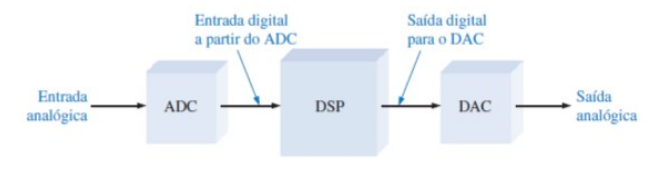
\includegraphics[scale=0.6]{fig/figura1.png}
    \label{figura:diagrama1}
    \caption{Diagrama em bloco básico de um sistema de processamento de sinais digitais}
\end{figure}

\paragraph{} Isto quer dizer que, a cada intervalo de tempo previamente definido é retirada uma amostra do sinal de entrada que vai ser codificada em forma binária e este procedimento é aplicado sucessivamente a cada novo intervalo de tempo.

\paragraph{} Esta amostragem é transferida ao processador que efetuar os cálculos numéricos. Estes cálculos envolvem multiplicações e soma com constantes de seus termos - produtos. Os resultados desses cálculos produzidos pelo processador agora representam valores do sinal filtrado e podem ser reconstituídos através de um DAC, o qual irá converter o sinal filtrado em um sinal na forma analógica. Note que num filtro digital, o sinal é representado por uma sucessão de números, em lugar de uma tensão ou corrente.

\paragraph{} Os filtros digitais são parte importante do Processamento Digital de Sinais (PDS). Na realidade, o desempenho extraordinário deles é uma das razões fundamentais para a popularização do PDS (STEVEN, 1999).

\paragraph{} Existem várias vantagens advindas da utilização de filtros digitais, entre ela:

\begin{enumerate}
    \item Um filtro digital é programável, ou seja, a sua operação é determinada por um programa armazenado na memória do processador. Isto significa que o filtro digital pode ser mudado facilmente sem afetar seu circuito eletrônico (hardware). No caso de um filtro analógico ocorre somente se mudarmos o seu circuito eletrônico;
    
    \item Os filtros digitais são facilmente projetados, sendo os mesmos testados e implementados em um computador ou estação de trabalho de forma simples;
    
    \item  As características funcionais dos circuitos de filtros analógicos (particularmente os circuitos elaborados com componentes) estão sujeitos a variação da temperatura, variação de valores devido à construção dos componentes utilizados nos circuitos, entre outros parâmetros que dependem do projeto e aplicação. Filtros digitais não sofrem estes problemas, logo são extremamente estáveis obtendo com isso resultados mais precisos.
\end{enumerate}

\paragraph{} A ordem de um filtro digital é o número de contribuições previamente armazenadas na memória do processador utilizadas para calcular a próxima componente. Sendo assim, todos os filtros digitais podem ser escritos da seguinte maneira:

\textbf{Zero - ordem}
\begin{equation}
y(n) = a_0x_n
\end{equation}

\textbf{Primeira - ordem}
\begin{equation}
y(n) = a_0x_n + a_1x_{n-1}
\end{equation}

\textbf{Segunda - ordem}
\begin{equation}
y(n) = a_0x_n + a_1x_{n-1} + a_2x_{n-2}
\end{equation}

\paragraph{} Filtros Digitais com ordens superiores a segunda podem ser desenvolvidos usando expressões semelhantes. As componentes \textbf{a0, a1, a2,..., an} são chamadas de “Coeficientes de Filtro”. Os valores desses coeficientes é que determinam as características do filtro em particular.

\paragraph{} Outra característica muito importante nos filtros digitais é a sua Função de Transferência. Esta função é obtida pela simetria da expressão do filtro, que nos permite descrever um filtro por meio de uma expressão conveniente e compacta. Pode-se usar a função de transferência de um filtro para trabalhar fora de sua resposta de frequência.

\paragraph{} Os filtros são divididos em duas categorias: Filtro de resposta ao impulso finito (FIR), também conhecido como filtro de média móvel (MA) e Filtro de resposta ao impulso infinito (IIR), também conhecido como filtro de média móvel autorregressiva (ARMA). 
\paragraph{} Um impulso é um sinal de curta duração que vai de zero a um valor máximo e volta a zero novamente em um curto espaço de tempo. A resposta ao impulso de um filtro é a resposta do filtro a um impulso e depende dos valores sobre os quais o filtro opera. Figura 2 ilustra a resposta ao impulso.

\begin{figure}[!htb]
    \centering
    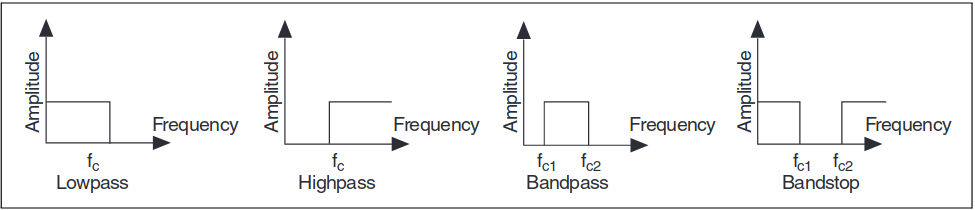
\includegraphics[scale=0.4]{fig/figura2.png}
    \label{figura:grafico}
    \caption{Resposta ao Impulso}
\end{figure}

\paragraph{} A transformada de Fourier da resposta ao impulso é a resposta em frequência do filtro. A resposta de frequência de um filtro fornece informações sobre a saída do filtro em diferentes frequência. Em outras palavras, a resposta de frequência de um filtro reflete o ganho do filtro em diferentes frequência. Para um filtro ideal, o ganho é um na banda passante e zero na banda final. Um filtro ideal passa todas as frequências na banda passante para a saída inalterada, mas não passa nenhuma das frequências na banda limite para a saída.

\subsection{Filtro FIR}
\paragraph{} Os filtros de resposta ao impulso finito (FIR) são filtros digitais que têm uma resposta de impulso finita. Os filtros FIR operam apenas nos valores de entrada atuais e passados e são os filtros mais simples de projetar. Os filtros FIR também são conhecidos como filtros não-recursivos, filtros de convolução e filtros de média móvel (MA). Os filtros FIR realizam uma convolução dos coeficientes do filtro com uma sequência de valores de entrada e produzem uma sequência igualmente numerada de valores de saída. A equação 4 define a equação de diferença que um filtro FIR executa.\\

\textbf{Equação de Diferença}
\begin{equation}
y[n] = b_0x[n] + b_1x[n-1] + ... + b_mx[n-m]
\end{equation}

\textbf{Função de Transferência}
\begin{equation}
H(z) = b_0 + b_1z^{-1} + ... + b_nz^{-n}
\end{equation}

\textbf{Resposta em Frequência}
\begin{equation}
H(e^{j\Omega}) = b_0 + b_1e^{-j\Omega} + ... + b_ne^{-j\Omega n}
\end{equation}

\textbf{Resposta ao Impulso}
\begin{equation}
h[n] = b_0\delta + b_1\delta[n-1] + ... + b_m\delta[n-m]
\end{equation}

\paragraph{} Os filtros FIR possuem as seguintes características:
\begin{enumerate}
    \item Possui resposta ao impulso finita. 
    \item São Bibos estáveis.
    \item Implementam resposta em fase linear.
    \\
\end{enumerate}

\paragraph{} Abaixo, na Figura 3, encontra-se a estrutura básica de um filtro FIR.

\begin{figure}[!htb]
    \centering
    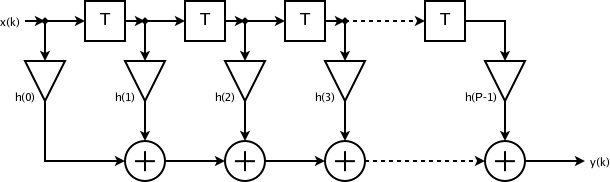
\includegraphics[scale=0.5]{fig/figura3.png}
    \label{figura:diagrama2}
    \caption{Estrutura Básica de um Filtro FIR}
\end{figure}

\paragraph{} Há situações em que o sinal analógico com características periódicas pode apresentar anormalidade em uma das extremidades após a aplicação da Transformada de Fourier, resultando em descontinuidades nas suas extremidades.
\paragraph{} Janelamento, ou simplesmente janela, é a técnica para aumentar as características espectrais de um sinal amostrado, esta técnica minimiza as margens de transição em formas de ondas truncadas.
\paragraph{} A janela consiste em aplicar uma função matemática, que depende do tipo de janela, ao sinal. O espectro de um sinal após o janelamento é o resultado da convolução do espectro do sinal original com o espectro da janela. Há vários tipos de janelas, apresentadas logo a seguir, e uso de um determinado tipo de janela dependerá da aplicação a ser filtrada.

\subsubsection{Métodos das janelas Retangular}
\paragraph{} A janela retangular possui valor igual a 1 em todo o seu intervalo de tempo. É a janela com maior perda espectral. Indicada para análise de transientes com duração menor que a da janela em análise.

\subsubsection{Métodos das janelas Triangular}
\paragraph{} A janela de Bartlett (Fejer, Cesaro ou como mais conhecidamente triangular) é inferior se comparada a janela de Hanning. Como o próprio nome indica a sua forma é de uma onda triangular.

\subsubsection{Métodos das janelas Hanning}
\paragraph{} Possui forma similar ao meio ciclo de uma onda cossenoidal e é útil para análise de transientes maiores que o tempo de duração da janela, bem como para aplicações de objetivos gerais. A janela Hanning força as extremidades ao valor zero.

\subsubsection{Métodos das janelas Hamming}
\paragraph{} Geralmente a mais utilizada de todas, a janela de Hamming possui a menor magnitude do lóbulo lateral para uma dada largura de lóbulo principal. Possui forma quase idêntica a da janela de Hanning, entretanto as extremidades da janela de Hamming não se aproximam do zero.

\subsection{Filtro IIR}
\paragraph{} Os filtros de resposta ao impulso infinito (IIR), também conhecidos como filtros recursivos e filtros de média móvel autorregressiva (ARMA), operam com valores de entrada atuais e passados e valores de saída atuais e passados. A resposta ao impulso de um filtro IIR é a resposta do filtro geral IIR a um impulso. Teoricamente, a resposta ao impulso de um filtro IIR nunca chega a zero e é uma resposta infinita. A seguinte equação de diferença geral caracteriza os filtros IIR.\\

\textbf{Equação de Diferença}
\begin{equation}
b_0x[n] + b_1x[n-1] + ... + b_mx[n-m] = y[n] + a_1y[n-1] + ... + a_my[n-m]
\end{equation}

\textbf{Função de Transferência}
\begin{equation}
H(z) = \frac{b_0 + b_1z^{-1} + ... + b_mz^{-m}}{1 + a_1z^{-1} + ... + a_nz^{-n}}
\end{equation}

\textbf{Resposta em Frequência}
\begin{equation}
H(e^{j\Omega}) = \frac{b_0 + b_1e^{-j\Omega} + ... + b_me^{-j\Omega m}}{1 + a_1e^{-j\Omega} + ... + a_ne^{-j\Omega n}}
\end{equation}

\paragraph{} Os filtros IIR possuem as seguintes características:
\begin{enumerate}
    \item Possui resposta ao impulso infinita. 
    \item A estabilidade depende da posição dos pólos.
    \item Não implementam resposta em fase linear.
    \item Para um mesmo grau de aproximação, precisam de uma ordem menor em comparação a um FIR.
    \\
\end{enumerate}

\paragraph{} Abaixo, na Figura 4, encontra-se a estrutura básica de um filtro IIR.

\begin{figure}[!htb]
    \centering
    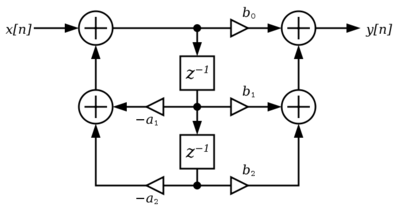
\includegraphics[scale=0.9]{fig/figura4.png}
    \label{figura:diagrama3}
    \caption{Estrutura Básica de um Filtro IIR}
\end{figure}

\subsubsection{Butterworth}
\paragraph{} O filtro Butterworth é um tipo de projeto de filtros eletrônicos. Ele é desenvolvido de modo a ter uma resposta em frequência o mais plana o quanto for matematicamente possível na banda passante(menor ripple).

\paragraph{} Os filtros Butterworth têm as seguintes características:
\begin{enumerate}
    \item Resposta suave em todas as frequência. 
    \item Diminuição monotônica das frequência de corte especificadas.
    \item Planicidade máxima, com a resposta ideal de unidade na banda passante e zero na banda de parada.
    \item frequência de meia potência ou 3 dB baixa frequência, que corresponde às frequência de corte especificadas. A vantagem dos filtros Butterworth é sua resposta de frequência suave e monotônica decrescente.
\end{enumerate}{}

\paragraph{} A figura 5 mostra a resposta de frequência de um filtro Butterworth lowpass.

\begin{figure}[!htb]
    \centering
    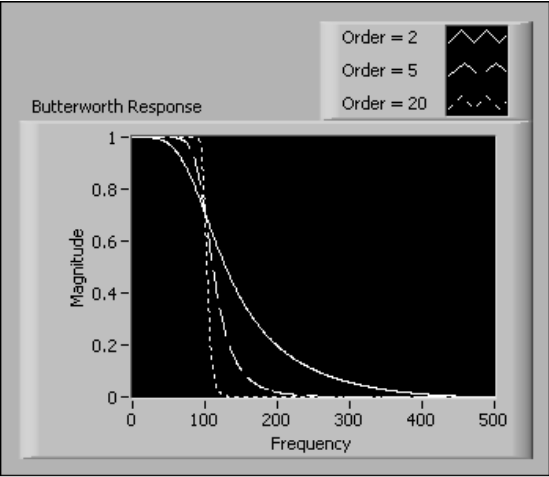
\includegraphics[scale=0.6]{fig/figura5.png}
    \label{figura:figura1}
    \caption{Resposta de Frequência de um Filtro Lowpass Butterworth}
\end{figure}

\paragraph{} Os filtros Butterworth nem sempre fornecem uma boa aproximação da resposta ideal do filtro, devido à lenta rolagem entre a banda passante e a banda de parada.

\subsubsection{Chebyshev I}
Os filtros Chebyshev são filtros analógicos ou digitais que possuem um aumento na atenuação (roll-off) e uma maior ondulação (ripple) na banda passante que os Filtros Butterworth. Os filtros Chebyshev possuem a propriedade de minimizarem o erro entre as características do filtro idealizado e o atual com relação à faixa do filtro, porém com ripples na banda passante. Este tipo de filtro recebeu seu nome em honra a Pafnuty Chebyshev, devido a suas características matemáticas serem derivadas dos polinômios de Chebyshev.

\paragraph{} Os filtros Chebyshev possuem as seguintes características:
\begin{enumerate}
    \item Minimização do erro de pico na faixa de passagem.
    \item Resposta de magnitude Equiripple na banda passante.
    \item Resposta de magnitude decrescente monotônica na banda de parada.
    \item Rolloff mais nítido que os filtros Butterworth.
\end{enumerate}{}

\paragraph{} Comparado a um filtro Butterworth, um filtro Chebyshev pode alcançar uma transição mais nítida entre a banda passante e a banda de parada com um filtro de ordem inferior. A transição brusca entre a banda passante e a banda de parada de um filtro Chebyshev produz menores erros absolutos e velocidades de execução mais rápidas do que um filtro Butterworth.

\paragraph{} A figura 6 mostra a resposta de frequência de um filtro Chebyshev lowpass.

\begin{figure}[!htb]
    \centering
    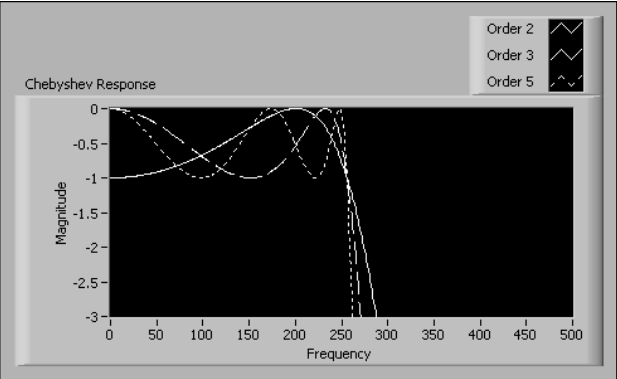
\includegraphics[scale=0.5]{fig/figura6.png}
    \label{figura:figura2}
    \caption{Resposta de Frequência de um Filtro Chebyshev Lowpass}
\end{figure}

\paragraph{} O erro máximo tolerável restringe a resposta equivocada na banda passante. Além disso, o roll off nítido aparece na banda de parada.

\subsubsection{Chebyshev II}
\paragraph{} Também conhecidos como Chebyshev invertidos, este tipo é menos comum pois ele não apresenta um roll off tão acentuado quanto o tipo I, e requer uma maior quantidade de componentes. Ele não possui ripple em sua banda passante, porém possui ripple na sua banda atenuada.

\paragraph{} Os filtros Chebyshev II possuem as seguintes características:
\begin{enumerate}
    \item Minimização do erro de pico na banda de parada.
    \item Resposta de magnitude Equiripple no stopband.
    \item Resposta de magnitude decrescente monotônica na faixa de passagem.
    \item Roll off mais nítido que os filtros Butterworth.
\end{enumerate}

\paragraph{} Os filtros Chebyshev II são semelhantes aos filtros Chebyshev. No entanto, os filtros Chebyshev II diferem dos filtros Chebyshev das seguintes maneiras:

\begin{enumerate}
    \item Os filtros Chebyshev II minimizam o erro de pico na banda de parada em vez da banda passante. Minimizar o erro de pico na banda de parada em vez da banda passante é uma vantagem dos filtros Chebyshev II sobre os filtros Chebyshev.
    \item Os filtros Chebyshev II têm uma resposta de magnitude equivocada na banda de interrupção, em vez da banda passante.
    \item Os filtros Chebyshev II têm uma resposta de magnitude monotonicamente decrescente na faixa de passagem em vez da banda de parada.
\end{enumerate}

\newpage
\paragraph{} A figura 7 mostra a resposta de frequência de um filtro Chebyshev II lowpass.

\begin{figure}[!htb]
    \centering
    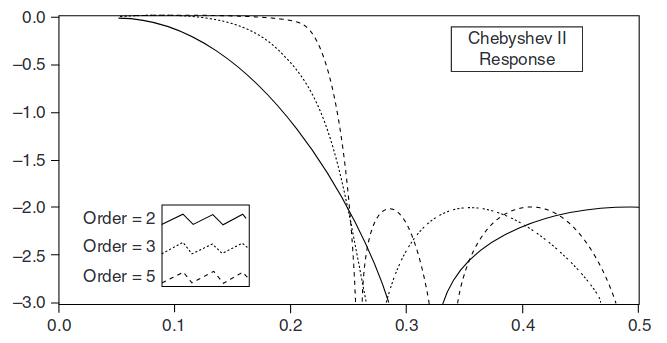
\includegraphics[scale=0.6]{fig/figura7.png}
    \label{figura:figura3}
    \caption{Resposta de Frequência de um Filtro Chebyshev II Lowpass}
\end{figure}

\paragraph{} O erro máximo tolerável restringe a resposta equivocada na banda de parada. Além disso, o suave rolloff monótono aparece no stopband.

\paragraph{} Os filtros Chebyshev II têm a mesma vantagem sobre os filtros Butterworth que os filtros Chebyshev têm - uma transição mais nítida entre a banda passante e a banda de parada com um filtro de ordem inferior, resultando em um erro absoluto menor e velocidade de execução mais rápida.

\subsubsection{Elíptico}
\paragraph{} Um filtro elíptico (também conhecido como filtro de Cauer) é um filtro com ondulações (ripple) na banda passante e na banda rejeitada. 

\paragraph{} Os filtros elípticos possuem as seguintes características:
\begin{enumerate}
    \item Minimização do erro de pico na banda passante e na banda de parada.
    \item Equivalentes na banda passante e na banda de parada.
    \\
\end{enumerate}
\newpage
\paragraph{} Comparados com os mesmos filtros Butterworth ou Chebyshev, os filtros elípticos fornecem a transição mais nítida entre a faixa de passagem e a banda de parada, o que explica seu amplo uso.
\\
\paragraph{} A figura 8 mostra a resposta de frequência de um filtro elíptico de baixa passagem.

\begin{figure}[!htb]
    \centering
    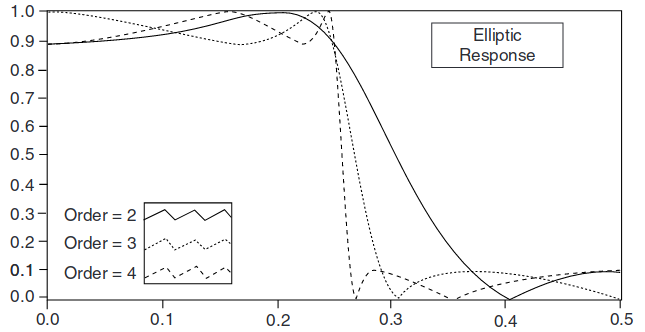
\includegraphics[scale=0.6]{fig/figura8.png}
    \label{figura:figura4}
    \caption{Resposta de Frequência de um Filtro Elíptico Lowpass}
\end{figure}

\paragraph{} O mesmo erro máximo tolerável restringe a ondulação na banda passante e na banda de parada. Além disso, mesmo os filtros elípticos de baixa ordem têm uma borda de transição nítida.
\newpage
\paragraph{} Aqui temos na figura 9, uma imagem mostrando a resposta em frequência do filtro elíptico ao lado das respostas de outros tipos comuns de filtros obtidos com o mesmo número de coeficientes: 

\begin{figure}[!htb]
    \centering
    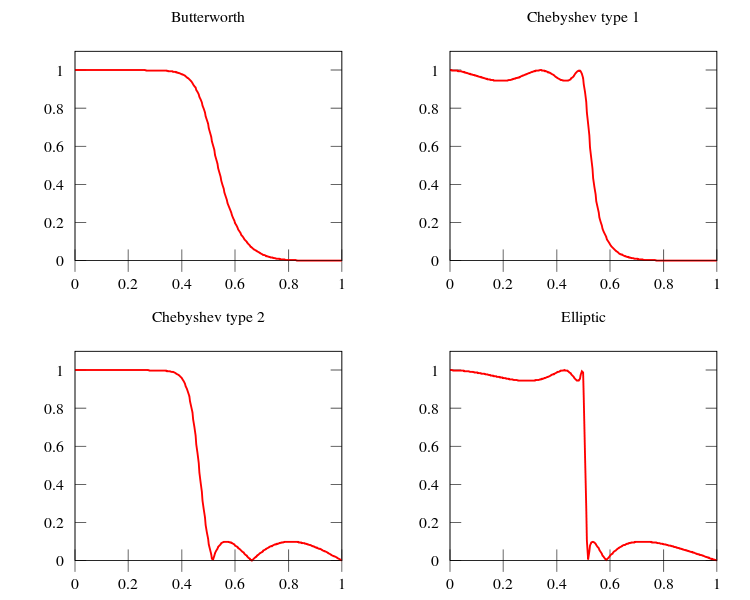
\includegraphics[scale=0.6]{fig/figura9.png}
    \label{figura:figura5}
    \caption{Comparação das Respostas em Frequência dos Filtros}
\end{figure}

\subsubsection{Notch}
\paragraph{} Um filtro Notch, também conhecido como rejeita-faixa ou filtro de rejeição de banda é um filtro que permite a passagem da maioria das frequências inalteradas, porém atenua aquelas que estejam em uma faixa determinada pelo filtro, ou seja elimina uma frequência específica. O princípio de funcionamento é o oposto do filtro passa-faixa.

\paragraph{} A figura 10 mostra a resposta de frequência de um filtro Notch.

\begin{figure}[!htb]
    \centering
    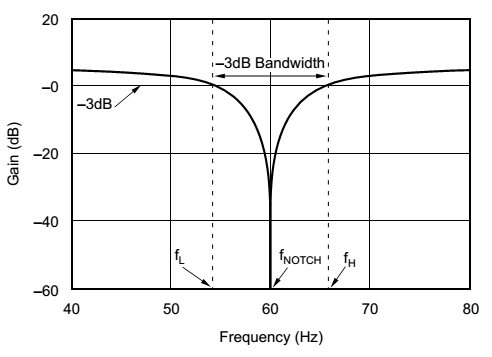
\includegraphics[scale=0.6]{fig/figura10.png}
    \label{figura:figura6}
    \caption{Resposta em Frequência do Filtro Notch}
\end{figure}

\subsubsection{Método da Transformação Bilinear}
\paragraph{} Os Planos S(analógica) e Z(usada em sistemas digitais) são ambos complexos. A Transformação Bilinear é um tipo de mapeamento conforme que mapeia pontos de um plano no outro. Os pontos sobre o eixo imaginário do Plano S são mapeados sobre círculo de raio unitário do Plano Z. A região à esquerda do eixo imaginário no Plano S é mapeada dentro do círculo de raio unitário no Plano Z.

\section{Metodologia e Apresentação de Resultados}
\paragraph{} O presente trabalho foi desenvolvido a partir de uma máquina com sistema operacional Linux de distribuição Mint 19.1, com uso de um software de processamento de sinais e sistema computacional e numérica, Octave na versão 4.2.2, para a aplicação dos filtros através de script.
\paragraph{} O presente áudio a ser trabalhado contém uma mistura de ruído, sirene e uma voz humana. Será analisado o espectro do sinal e utilizar os filtros digitais disponíveis para assim então obter um áudio filtrado sem os ruídos e sirene até que a voz humana fique mais clara e interpretada.

\subsection{Análise espectral e Projeto do Filtro IIR}
\paragraph{} O primeiro a passo a fazer é uma análise espectral, onde precisamos ler o arquivo de áudio em questão, armazenar e identificar os componentes de frequência da fala humana e suas interferências, logo após iremos jogar para o domínio da frequência e então normalizar a frequência.

\lstinputlisting[firstline=1,lastline=17]{codes/codigo1-IIR.m}
\paragraph{} Após a execução do código acima, obtemos a seguinte análise espectral, como mostrada pela figura 11 abaixo:

\begin{figure}[!htb]
    \centering
    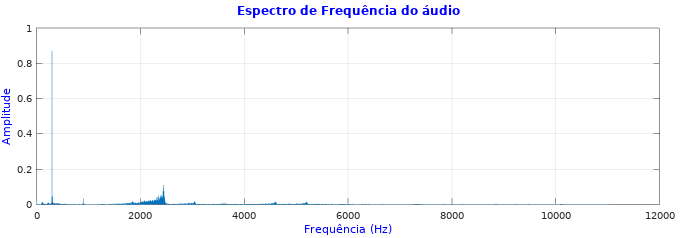
\includegraphics[scale=0.6]{fig/sinal1.png}
    \label{figura:figura7}
    \caption{Análise espectral do sinal de áudio}
\end{figure}

\paragraph{} Analisando o espectro do sinal, vemos que existe um pico de sinal anormal em 300Hz onde o mesmo será eliminado com a utilização do filtro Notch, pois é o mais recomendado. Segue abaixo o código para o filtro Notch:

\lstinputlisting[firstline=20,lastline=45]{codes/codigo1-IIR.m}
\newpage
\paragraph{} Após a execução do código acima, obtemos a seguinte resultado com a utilização do filtro Notch. Foram gerados dois gráficos, o gráfico superior contém o áudio original em conjunto com a linha de corte do filtro Notch já o gráfico inferior contém o espectro do sinal filtrado como será mostrada pela figura 12 abaixo:

\begin{figure}[!htb]
    \centering
    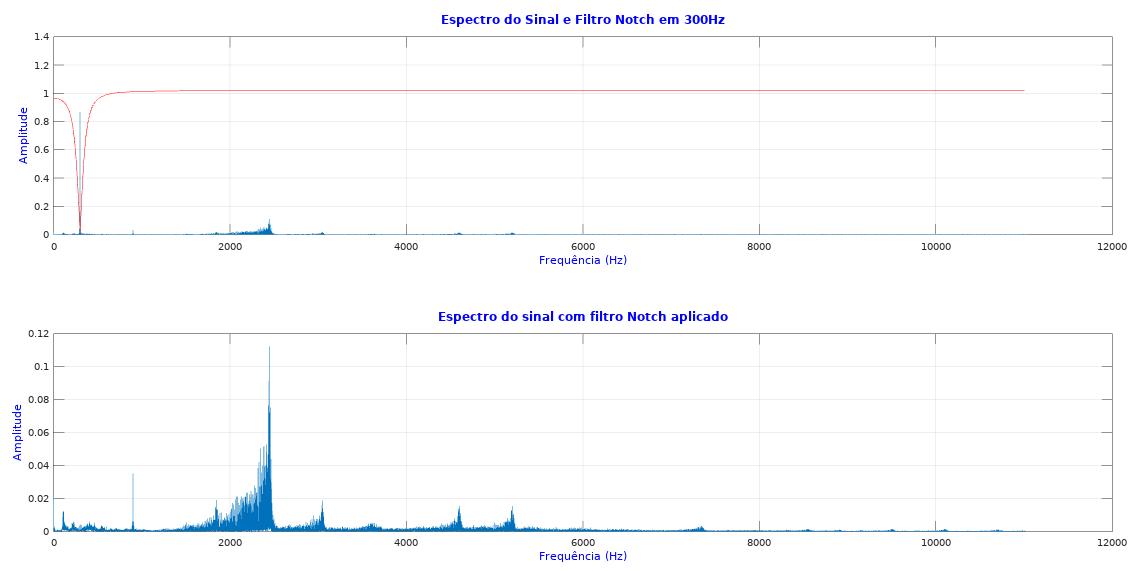
\includegraphics[scale=0.4]{fig/sinal2.png}
    \label{figura:figura8}
    \caption{Resultado do filtro Notch}
\end{figure}

\paragraph{} Após o processo da primeira filtragem com o filtro Notch, ainda podemos identificar outros componentes na frequência que devem ser eliminados, com isso utilizamos mais dois filtros, o filtro Butterworth Passa-Alta para eliminar as frequências abaixo da frequência de corte de 100Hz e o filtro Butterworth Passa-Baixa que irá eliminar a frequência de corte acima de 550Hz. O código abaixo mostra como foi efetuado o filtro.

\newpage

\lstinputlisting[firstline=50,lastline=64]{codes/codigo1-IIR.m}

\subsection{Resposta em Frequência e Resposta ao Impulso do Filtro}
\paragraph{} A figura 13 abaixo mostra o gráfico da Resposta em Frequência, ou seja o resultado do processo de filtragem dos três filtros.

\begin{figure}[!htb]
    \centering
    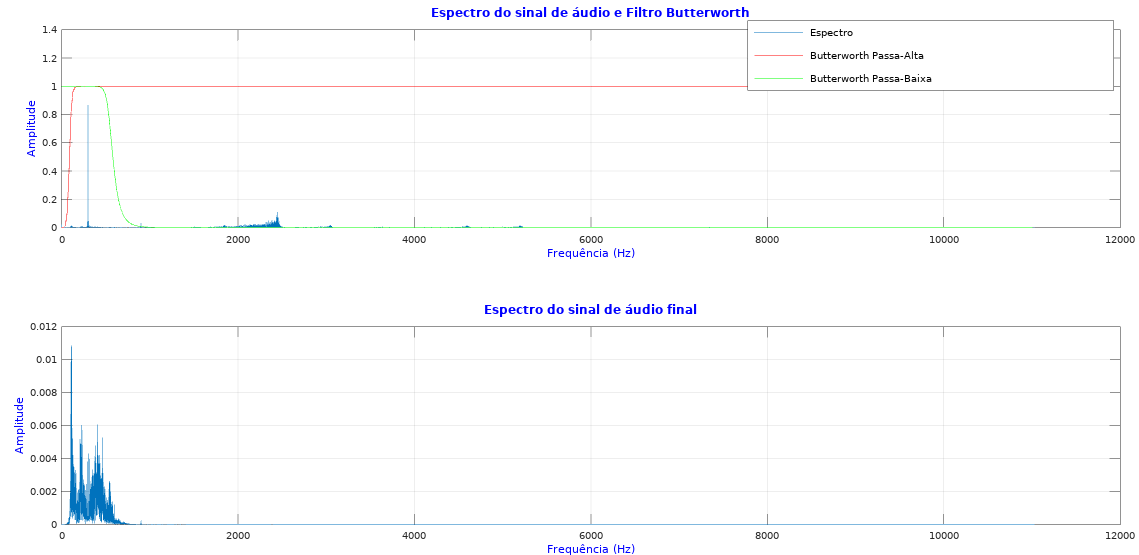
\includegraphics[scale=0.4]{fig/sinal3.png}
    \label{figura:figura9}
    \caption{Espectro do sinal de áudio e Espectro do sinal final}
\end{figure}

\newpage

\paragraph{} A figura 14 abaixo mostra o gráfico da Resposta ao Impulso.

\begin{figure}[!htb]
    \centering
    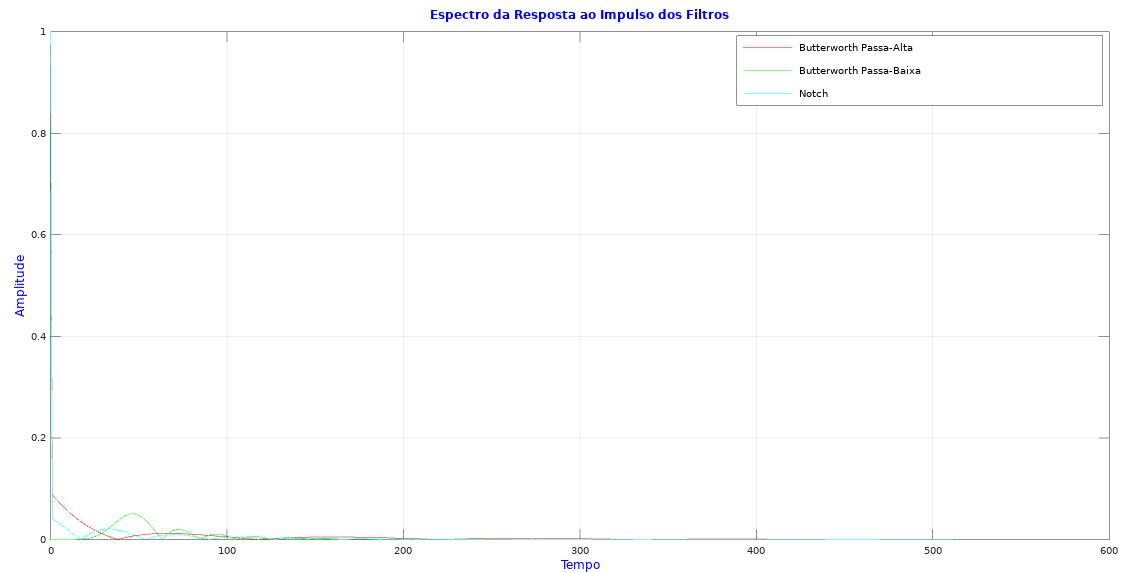
\includegraphics[scale=0.4]{fig/sinal4.png}
    \label{figura:figura10}
    \caption{Espectro da Resposta ao Impulso}
\end{figure}

\subsection{Coeficientes do Filtros}
\begin{enumerate}
    \item Filtro Notch:
    \\ Numerador: [  1.0000, -1.9927,  1.0000 ]
    \\ Denominador: [  1.00000, -1.95284,  0.96040 ]
    \item Filtro Butterworth Passa-Alta:
    \\ Numerador: [  0.95494, -4.77469,  9.54939, -9.54939,  4.77469, -0.95494 ]
    \\ Denominador: [  1.00000, -4.90779,  9.63539, -9.45932,  4.64363, -0.91191 ]
    \item Filtro Butterworth Passa-Baixa:
    \\ Numerador: [  5.3964e-12,  5.3964e-11,  2.4284e-10,  6.4756e-10,  1.1332e-09,  1.3599e-09,  1.1332e-09,  6.4756e-10,   2.4284e-10,  5.3964e-11,  5.3964e-12 ]
    \\ Denominador: [  1.00000,  -8.99822,  36.48154,  -87.75582,  138.69530, -150.48362,  113.51109,  -58.77613,  19.99357,  -4.03442,  0.36671 ]
\end{enumerate}

\subsection{Análise espectral e Projeto do Filtro FIR}
\paragraph{} Como já foi constatado em análise prévia já descrita para os filtros IIR, sabemos as frequências a serem eliminadas, resta apenas projetar o filtro do tipo FIR para cumprir esse objetivo. Foi utilizado dois filtros passa-banda, um na frequência de 100Hz a 200Hz e outro de 400Hz a 700Hz, ambos com ordem de 500. O código abaixo mostra o processo de filtragem.

\lstinputlisting[firstline=19,lastline=47]{codes/codigo2-FIR.m}

\newpage

\subsection{Resposta em Frequência e Resposta ao Impulso do filtro}
\paragraph{} A figura 15 mostra o gráfico da Resposta em Frequência, ou seja o resultado do processo de filtragem dos dois filtros e a figura 16 mostra o gráfico da Resposta ao Impulso.

\begin{figure}[!htb]
    \centering
    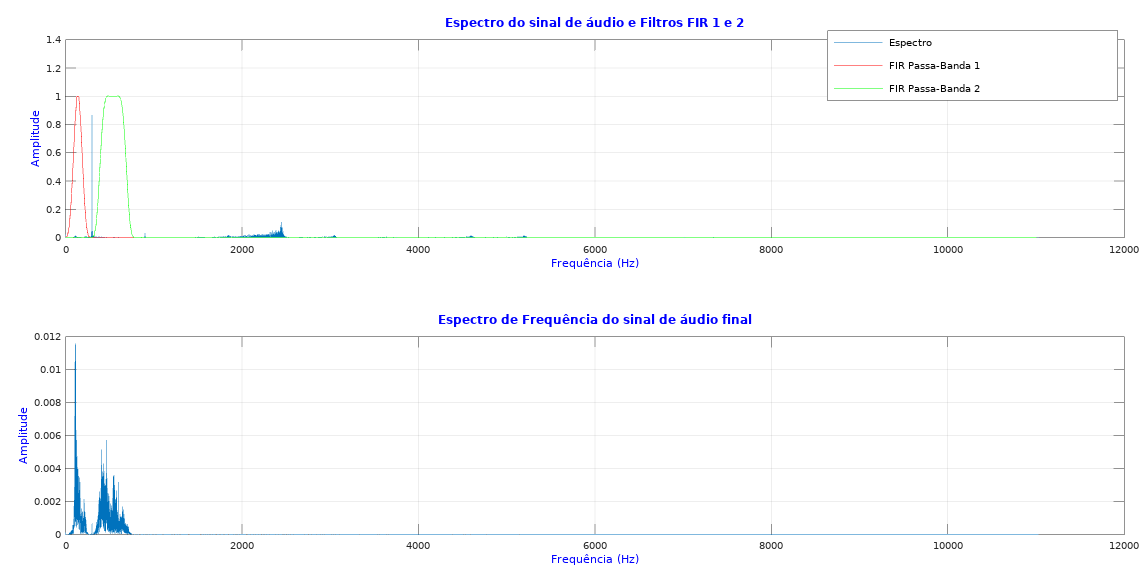
\includegraphics[scale=0.4]{fig/sinal5.png}
    \label{figura:figura11}
    \caption{Espectro da Resposta em Frequência}
\end{figure}

\begin{figure}[!htb]
    \centering
    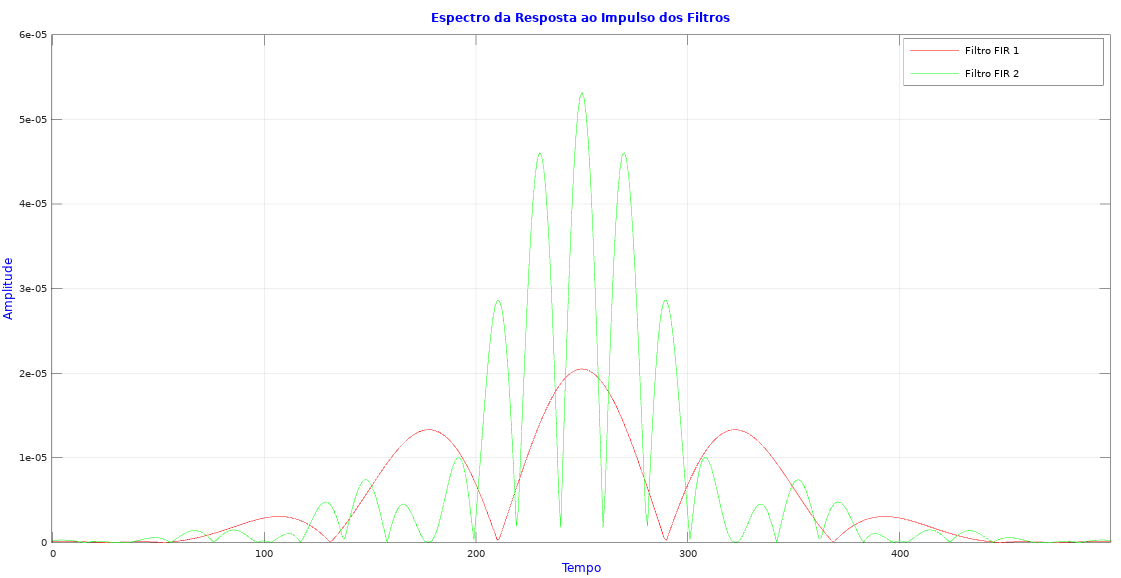
\includegraphics[scale=0.4]{fig/sinal6.png}
    \label{figura:figura12}
    \caption{Espectro da Resposta ao Impulso}
\end{figure}

\newpage
\subsection{Coeficientes do Filtros}

\begin{enumerate}
    \item FIR Passa-Banda 1:
    \\ Numerador: [  6.4223e-05,  6.3459e-05,  6.2542e-05,  6.1474e-05,  6.0258e-05,  5.8895e-05,  5.7386e-05,  5.5733e-05,  5.3937e-05,  5.2000e-05,  4.9921e-05,  4.7704e-05,  4.5349e-05,  4.2859e-05,  4.0236e-05,  3.7484e-05,  3.4606e-05,  3.1608e-05,  2.8495e-05,  2.5273e-05,  2.1951e-05,  1.8537e-05,  1.5043e-05,  1.1479e-05,  7.8596e-06,  4.1995e-06,  5.1533e-07, -3.1743e-06, -6.8493e-06, -1.0487e-05, -1.4064e-05, -1.7554e-05,  -2.0929e-05, -2.4160e-05, -2.7213e-05, -3.0056e-05, -3.2653e-05, -3.4966e-05, -3.6956e-05, -3.8583e-05,  -3.9803e-05, -4.0572e-05, -4.0846e-05, -4.0578e-05, -3.9721e-05, -3.8225e-05, -3.6042e-05, -3.3123e-05,  -2.9418e-05, -2.4877e-05, -1.9451e-05, -1.3091e-05, -5.7495e-06,  2.6212e-06,  1.2066e-05,  2.2630e-05,  3.4353e-05,  4.7276e-05,  6.1436e-05,  7.6866e-05,  9.3597e-05,  1.1166e-04,  1.3107e-04,  1.5185e-04,  1.7401e-04,  1.9757e-04,  2.2252e-04,  2.4887e-04,  2.7660e-04,  3.0571e-04,  3.3618e-04,  3.6797e-04,  4.0106e-04,  4.3540e-04,  4.7094e-04,  5.0764e-04,  5.4543e-04,  5.8423e-04,  6.2397e-04,  6.6456e-04,  7.0591e-04,  7.4792e-04,  7.9047e-04,  8.3346e-04,  8.7674e-04,  9.2020e-04,  9.6368e-04,  1.0070e-03,  1.0501e-03,  1.0928e-03,  1.1348e-03,  1.1761e-03,  1.2164e-03,  1.2556e-03,  1.2934e-03,  1.3297e-03,  1.3643e-03,  1.3969e-03,  1.4274e-03,  1.4555e-03,  1.4811e-03,  1.5040e-03,  1.5238e-03,  1.5405e-03,  1.5537e-03,  1.5634e-03,  1.5693e-03,  1.5711e-03,  1.5688e-03,  1.5620e-03,  1.5507e-03,  1.5346e-03,  1.5136e-03,  1.4874e-03,  1.4561e-03,  1.4193e-03,  1.3770e-03,  1.3290e-03,  1.2753e-03,  1.2157e-03,  1.1502e-03,  1.0787e-03,  1.0011e-03,  9.1744e-04,  8.2763e-04,  7.3170e-04,  6.2965e-04,  5.2152e-04,  4.0735e-04,  2.8722e-04,  1.6121e-04,  2.9425e-05, -1.0800e-04, -2.5093e-04, -3.9920e-04, -5.5261e-04,  -7.1097e-04, -8.7404e-04, -1.0416e-03, -1.2133e-03, -1.3890e-03, -1.5683e-03, -1.7509e-03, -1.9365e-03,  -2.1246e-03, -2.3150e-03, -2.5072e-03, -2.7009e-03, -2.8956e-03, -3.0908e-03, -3.2862e-03, -3.4812e-03,  -3.6754e-03, -3.8684e-03, -4.0596e-03, -4.2485e-03, -4.4347e-03, -4.6176e-03, -4.7966e-03, -4.9714e-03,  -5.1414e-03, -5.3060e-03, -5.4648e-03, -5.6173e-03, -5.7629e-03, -5.9011e-03, -6.0315e-03, -6.1535e-03,  -6.2668e-03, -6.3708e-03, -6.4651e-03, -6.5493e-03, -6.6229e-03, -6.6856e-03, -6.7370e-03, -6.7768e-03,  -6.8045e-03, -6.8199e-03, -6.8228e-03, -6.8127e-03, -6.7896e-03, -6.7533e-03, -6.7034e-03, -6.6400e-03,  -6.5628e-03, -6.4719e-03, -6.3670e-03, -6.2483e-03, -6.1158e-03, -5.9694e-03, -5.8093e-03, -5.6356e-03,  -5.4484e-03, -5.2479e-03, -5.0344e-03, -4.8080e-03, -4.5691e-03, -4.3181e-03, -4.0551e-03, -3.7807e-03,  -3.4953e-03, -3.1992e-03, -2.8930e-03, -2.5772e-03, -2.2523e-03, -1.9189e-03, -1.5775e-03, -1.2289e-03,  -8.7353e-04, -5.1218e-04, -1.4550e-04,  2.2582e-04,  6.0106e-04,  9.7948e-04,  1.3603e-03,  1.7429e-03,  2.1263e-03,  2.5099e-03,  2.8928e-03,  3.2743e-03,  3.6535e-03,  4.0297e-03,  4.4021e-03,  4.7699e-03,  5.1323e-03,  5.4885e-03,  5.8378e-03,  6.1794e-03,  6.5125e-03,  6.8365e-03,  7.1507e-03,  7.4543e-03,  7.7466e-03,  8.0271e-03,  8.2951e-03,  8.5500e-03,  8.7913e-03,  9.0184e-03,  9.2307e-03,  9.4279e-03,  9.6095e-03,  9.7750e-03,  9.9242e-03,  1.0057e-02,  1.0172e-02,  1.0270e-02,  1.0351e-02,  1.0413e-02,  1.0458e-02,  1.0485e-02,  1.0494e-02,  1.0485e-02,  1.0458e-02,  1.0413e-02,  1.0351e-02,  1.0270e-02,  1.0172e-02,  1.0057e-02,  9.9242e-03,  9.7750e-03,  9.6095e-03,  9.4279e-03,  9.2307e-03,  9.0184e-03,  8.7913e-03,  8.5500e-03,  8.2951e-03,  8.0271e-03,  7.7466e-03,  7.4543e-03,  7.1507e-03,  6.8365e-03,  6.5125e-03,  6.1794e-03,  5.8378e-03,  5.4885e-03,  5.1323e-03,  4.7699e-03,  4.4021e-03,  4.0297e-03,  3.6535e-03,  3.2743e-03,  2.8928e-03,  2.5099e-03,  2.1263e-03,  1.7429e-03,  1.3603e-03,  9.7948e-04,  6.0106e-04,  2.2582e-04, -1.4550e-04, -5.1218e-04, -8.7353e-04, -1.2289e-03, -1.5775e-03, -1.9189e-03,  -2.2523e-03, -2.5772e-03, -2.8930e-03, -3.1992e-03, -3.4953e-03, -3.7807e-03, -4.0551e-03, -4.3181e-03,  -4.5691e-03, -4.8080e-03, -5.0344e-03, -5.2479e-03, -5.4484e-03, -5.6356e-03, -5.8093e-03, -5.9694e-03,  -6.1158e-03, -6.2483e-03, -6.3670e-03, -6.4719e-03, -6.5628e-03, -6.6400e-03, -6.7034e-03, -6.7533e-03,  -6.7896e-03, -6.8127e-03, -6.8228e-03, -6.8199e-03, -6.8045e-03, -6.7768e-03, -6.7370e-03, -6.6856e-03,  -6.6229e-03, -6.5493e-03, -6.4651e-03, -6.3708e-03, -6.2668e-03, -6.1535e-03, -6.0315e-03, -5.9011e-03,  -5.7629e-03, -5.6173e-03, -5.4648e-03, -5.3060e-03, -5.1414e-03, -4.9714e-03, -4.7966e-03, -4.6176e-03,  -4.4347e-03, -4.2485e-03, -4.0596e-03, -3.8684e-03, -3.6754e-03, -3.4812e-03, -3.2862e-03, -3.0908e-03,  -2.8956e-03, -2.7009e-03, -2.5072e-03, -2.3150e-03, -2.1246e-03, -1.9365e-03, -1.7509e-03, -1.5683e-03,  -1.3890e-03, -1.2133e-03, -1.0416e-03, -8.7404e-04, -7.1097e-04, -5.5261e-04, -3.9920e-04, -2.5093e-04,  -1.0800e-04,  2.9425e-05,  1.6121e-04,  2.8722e-04,  4.0735e-04,  5.2152e-04,  6.2965e-04,  7.3170e-04,  8.2763e-04,  9.1744e-04,  1.0011e-03,  1.0787e-03,  1.1502e-03,  1.2157e-03,  1.2753e-03,  1.3290e-03,  1.3770e-03,  1.4193e-03,  1.4561e-03,  1.4874e-03,  1.5136e-03,  1.5346e-03,  1.5507e-03,  1.5620e-03,  1.5688e-03,  1.5711e-03,  1.5693e-03,  1.5634e-03,  1.5537e-03,  1.5405e-03,  1.5238e-03,  1.5040e-03,  1.4811e-03,  1.4555e-03,  1.4274e-03,  1.3969e-03,  1.3643e-03,  1.3297e-03,  1.2934e-03,  1.2556e-03,  1.2164e-03,  1.1761e-03,  1.1348e-03,  1.0928e-03,  1.0501e-03,  1.0070e-03,  9.6368e-04,  9.2020e-04,  8.7674e-04,  8.3346e-04,  7.9047e-04,  7.4792e-04,  7.0591e-04,  6.6456e-04,  6.2397e-04,  5.8423e-04,  5.4543e-04,  5.0764e-04,  4.7094e-04,  4.3540e-04,  4.0106e-04,  3.6797e-04,  3.3618e-04,  3.0571e-04,  2.7660e-04,  2.4887e-04,  2.2252e-04,  1.9757e-04,  1.7401e-04,  1.5185e-04,  1.3107e-04,  1.1166e-04,  9.3597e-05,  7.6866e-05,  6.1436e-05,  4.7276e-05,  3.4353e-05,  2.2630e-05,  1.2066e-05,  2.6212e-06,  -5.7495e-06, -1.3091e-05, -1.9451e-05, -2.4877e-05, -2.9418e-05, -3.3123e-05, -3.6042e-05, -3.8225e-05,  -3.9721e-05, -4.0578e-05, -4.0846e-05, -4.0572e-05, -3.9803e-05, -3.8583e-05, -3.6956e-05, -3.4966e-05,  -3.2653e-05, -3.0056e-05, -2.7213e-05, -2.4160e-05, -2.0929e-05, -1.7554e-05, -1.4064e-05, -1.0487e-05,  -6.8493e-06, -3.1743e-06,  5.1533e-07,  4.1995e-06,  7.8596e-06,  1.1479e-05,  1.5043e-05,  1.8537e-05,  2.1951e-05,  2.5273e-05,  2.8495e-05,  3.1608e-05,  3.4606e-05,  3.7484e-05,  4.0236e-05,  4.2859e-05,  4.5349e-05,  4.7704e-05,  4.9921e-05,  5.2000e-05,  5.3937e-05,  5.5733e-05,  5.7386e-05,  5.8895e-05,  6.0258e-05,  6.1474e-05,  6.2542e-05,  6.3459e-05,  6.4223e-05 ]
    \item FIR Passa-Banda 2:
    \\ Numerador: [ -1.1495e-04, -1.2830e-04, -1.3824e-04, -1.4458e-04, -1.4719e-04, -1.4607e-04, -1.4135e-04, -1.3323e-04,  -1.2203e-04, -1.0816e-04, -9.2115e-05, -7.4451e-05, -5.5770e-05, -3.6707e-05, -1.7902e-05,  1.9337e-08,  1.6467e-05,  3.0909e-05,  4.2897e-05,  5.2078e-05,  5.8218e-05,  6.1208e-05,  6.1078e-05,  5.8001e-05,  5.2285e-05,  4.4376e-05,  3.4836e-05,  2.4331e-05,  1.3605e-05,  3.4499e-06, -5.3223e-06, -1.1919e-05,  -1.5602e-05, -1.5725e-05, -1.1768e-05, -3.3750e-06,  9.6229e-06,  2.7181e-05,  4.9026e-05,  7.4651e-05,  1.0331e-04,  1.3405e-04,  1.6570e-04,  1.9694e-04,  2.2632e-04,  2.5231e-04,  2.7337e-04,  2.8801e-04,  2.9483e-04,  2.9262e-04,  2.8041e-04,  2.5752e-04,  2.2360e-04,  1.7871e-04,  1.2330e-04,  5.8244e-05,  -1.5148e-05, -9.5181e-05, -1.7979e-04, -2.6662e-04, -3.5304e-04, -4.3629e-04, -5.1354e-04, -5.8198e-04,  -6.3895e-04, -6.8205e-04, -7.0919e-04, -7.1875e-04, -7.0961e-04, -6.8124e-04, -6.3373e-04, -5.6782e-04,  -4.8491e-04, -3.8701e-04, -2.7671e-04, -1.5707e-04, -3.1581e-05,  9.6011e-05,  2.2180e-04,  3.4188e-04,  4.5250e-04,  5.5017e-04,  6.3185e-04,  6.9505e-04,  7.3796e-04,  7.5952e-04,  7.5945e-04,  7.3836e-04,  6.9764e-04,  6.3949e-04,  5.6683e-04,  4.8317e-04,  3.9248e-04,  2.9905e-04,  2.0728e-04,  1.2150e-04,  4.5791e-05, -1.6232e-05, -6.1589e-05, -8.8090e-05, -9.4467e-05, -8.0468e-05, -4.6913e-05,  4.2997e-06,  7.0229e-05,  1.4698e-04,  2.2982e-04,  3.1339e-04,  3.9186e-04,  4.5922e-04,  5.0953e-04,  5.3717e-04,  5.3714e-04,  5.0531e-04,  4.3867e-04,  3.3553e-04,  1.9568e-04,  2.0510e-05, -1.8696e-04, -4.2207e-04,  -6.7862e-04, -9.4901e-04, -1.2245e-03, -1.4953e-03, -1.7512e-03, -1.9817e-03, -2.1764e-03, -2.3257e-03,  -2.4206e-03, -2.4539e-03, -2.4197e-03, -2.3144e-03, -2.1366e-03, -1.8871e-03, -1.5695e-03, -1.1898e-03,  -7.5620e-04, -2.7932e-04,  2.2843e-04,  7.5307e-04,  1.2796e-03,  1.7922e-03,  2.2753e-03,  2.7136e-03,  3.0930e-03,  3.4007e-03,  3.6264e-03,  3.7618e-03,  3.8019e-03,  3.7444e-03,  3.5906e-03,  3.3448e-03,  3.0145e-03,  2.6103e-03,  2.1451e-03,  1.6344e-03,  1.0948e-03,  5.4420e-04,  8.5996e-07, -5.1743e-04,  -9.9390e-04, -1.4135e-03, -1.7635e-03, -2.0340e-03, -2.2186e-03, -2.3142e-03, -2.3219e-03, -2.2461e-03,  -2.0954e-03, -1.8815e-03, -1.6191e-03, -1.3252e-03, -1.0187e-03, -7.1922e-04, -4.4651e-04, -2.1947e-04,  -5.5288e-05,  3.1388e-05,  2.9253e-05, -6.9003e-05, -2.6617e-04, -5.6013e-04, -9.4370e-04, -1.4047e-03,  -1.9259e-03, -2.4861e-03, -3.0599e-03, -3.6193e-03, -4.1342e-03, -4.5736e-03, -4.9071e-03, -5.1058e-03,  -5.1436e-03, -4.9986e-03, -4.6544e-03, -4.1004e-03, -3.3334e-03, -2.3578e-03, -1.1858e-03,  1.6196e-04,  1.6572e-03,  3.2643e-03,  4.9409e-03,  6.6392e-03,  8.3072e-03,  9.8904e-03,  1.1333e-02,  1.2581e-02,  1.3581e-02,  1.4287e-02,  1.4657e-02,  1.4659e-02,  1.4268e-02,  1.3472e-02,  1.2270e-02,  1.0673e-02,  8.7034e-03,  6.3978e-03,  3.8031e-03,  9.7715e-04, -2.0129e-03, -5.0924e-03, -8.1809e-03, -1.1195e-02,  -1.4049e-02, -1.6662e-02, -1.8952e-02, -2.0848e-02, -2.2286e-02, -2.3214e-02, -2.3590e-02, -2.3390e-02,  -2.2603e-02, -2.1235e-02, -1.9307e-02, -1.6859e-02, -1.3942e-02, -1.0624e-02, -6.9833e-03, -3.1098e-03,  8.9980e-04,  4.9435e-03,  8.9172e-03,  1.2717e-02,  1.6244e-02,  1.9405e-02,  2.2115e-02,  2.4301e-02,  2.5907e-02,  2.6888e-02,  2.7218e-02,  2.6888e-02,  2.5907e-02,  2.4301e-02,  2.2115e-02,  1.9405e-02,  1.6244e-02,  1.2717e-02,  8.9172e-03,  4.9435e-03,  8.9980e-04, -3.1098e-03, -6.9833e-03, -1.0624e-02,  -1.3942e-02, -1.6859e-02, -1.9307e-02, -2.1235e-02, -2.2603e-02, -2.3390e-02, -2.3590e-02, -2.3214e-02,  -2.2286e-02, -2.0848e-02, -1.8952e-02, -1.6662e-02, -1.4049e-02, -1.1195e-02, -8.1809e-03, -5.0924e-03,  -2.0129e-03,  9.7715e-04,  3.8031e-03,  6.3978e-03,  8.7034e-03,  1.0673e-02,  1.2270e-02,  1.3472e-02,  1.4268e-02,  1.4659e-02,  1.4657e-02,  1.4287e-02,  1.3581e-02,  1.2581e-02,  1.1333e-02,  9.8904e-03,  8.3072e-03,  6.6392e-03,  4.9409e-03,  3.2643e-03,  1.6572e-03,  1.6196e-04, -1.1858e-03, -2.3578e-03,  -3.3334e-03, -4.1004e-03, -4.6544e-03, -4.9986e-03, -5.1436e-03, -5.1058e-03, -4.9071e-03, -4.5736e-03,  -4.1342e-03, -3.6193e-03, -3.0599e-03, -2.4861e-03, -1.9259e-03, -1.4047e-03, -9.4370e-04, -5.6013e-04,  -2.6617e-04, -6.9003e-05,  2.9253e-05,  3.1388e-05, -5.5288e-05, -2.1947e-04, -4.4651e-04, -7.1922e-04,  -1.0187e-03, -1.3252e-03, -1.6191e-03, -1.8815e-03, -2.0954e-03, -2.2461e-03, -2.3219e-03, -2.3142e-03,  -2.2186e-03, -2.0340e-03, -1.7635e-03, -1.4135e-03, -9.9390e-04, -5.1743e-04,  8.5996e-07,  5.4420e-04,  1.0948e-03,  1.6344e-03,  2.1451e-03,  2.6103e-03,  3.0145e-03,  3.3448e-03,  3.5906e-03,  3.7444e-03,  3.8019e-03,  3.7618e-03,  3.6264e-03,  3.4007e-03,  3.0930e-03,  2.7136e-03,  2.2753e-03,  1.7922e-03,  1.2796e-03,  7.5307e-04,  2.2843e-04, -2.7932e-04, -7.5620e-04, -1.1898e-03, -1.5695e-03, -1.8871e-03,  -2.1366e-03, -2.3144e-03, -2.4197e-03, -2.4539e-03, -2.4206e-03, -2.3257e-03, -2.1764e-03, -1.9817e-03,  -1.7512e-03, -1.4953e-03, -1.2245e-03, -9.4901e-04, -6.7862e-04, -4.2207e-04, -1.8696e-04,  2.0510e-05,  1.9568e-04,  3.3553e-04,  4.3867e-04,  5.0531e-04,  5.3714e-04,  5.3717e-04,  5.0953e-04,  4.5922e-04,  3.9186e-04,  3.1339e-04,  2.2982e-04,  1.4698e-04,  7.0229e-05,  4.2997e-06, -4.6913e-05, -8.0468e-05,  -9.4467e-05, -8.8090e-05, -6.1589e-05, -1.6232e-05,  4.5791e-05,  1.2150e-04,  2.0728e-04,  2.9905e-04,  3.9248e-04,  4.8317e-04,  5.6683e-04,  6.3949e-04,  6.9764e-04,  7.3836e-04,  7.5945e-04,  7.5952e-04,  7.3796e-04,  6.9505e-04,  6.3185e-04,  5.5017e-04,  4.5250e-04,  3.4188e-04,  2.2180e-04,  9.6011e-05,  -3.1581e-05, -1.5707e-04, -2.7671e-04, -3.8701e-04, -4.8491e-04, -5.6782e-04, -6.3373e-04, -6.8124e-04,  -7.0961e-04, -7.1875e-04, -7.0919e-04, -6.8205e-04, -6.3895e-04, -5.8198e-04, -5.1354e-04, -4.3629e-04,  -3.5304e-04, -2.6662e-04, -1.7979e-04, -9.5181e-05, -1.5148e-05,  5.8244e-05,  1.2330e-04,  1.7871e-04,  2.2360e-04,  2.5752e-04,  2.8041e-04,  2.9262e-04,  2.9483e-04,  2.8801e-04,  2.7337e-04,  2.5231e-04,  2.2632e-04,  1.9694e-04,  1.6570e-04,  1.3405e-04,  1.0331e-04,  7.4651e-05,  4.9026e-05,  2.7181e-05,  9.6229e-06, -3.3750e-06, -1.1768e-05, -1.5725e-05, -1.5602e-05, -1.1919e-05, -5.3223e-06,  3.4499e-06,  1.3605e-05,  2.4331e-05,  3.4836e-05,  4.4376e-05,  5.2285e-05,  5.8001e-05,  6.1078e-05,  6.1208e-05,  5.8218e-05,  5.2078e-05,  4.2897e-05,  3.0909e-05,  1.6467e-05,  1.9337e-08, -1.7902e-05, -3.6707e-05,  -5.5770e-05, -7.4451e-05, -9.2115e-05, -1.0816e-04, -1.2203e-04, -1.3323e-04, -1.4135e-04, -1.4607e-04,  -1.4719e-04, -1.4458e-04, -1.3824e-04, -1.2830e-04, -1.1495e-04 ]
\end{enumerate}{}


\section{Conclusão}

\paragraph{} A primeira etapa do processo de filtragem, foi utilizado o Filtro IIR dos tipos de filtros Notch(Rejeita Faixa) e Butterworth(Passa-Alta/Passa-Baixa) resultou em um áudio sem o ruído ao fundo, ou seja a eliminação das interferências ruídos, porém foram identificadas uma sutil diferença em relação ao tom do áudio, bem como a sua intensidade, mas foi resolvido amplificando o sinal antes de gerar. A segunda etapa foi utilizado o filtro FIR, que também tinha como objetivo eliminar o áudio da sirene/interferências e deixar somente a voz humana. O áudio resultante de ambos métodos de filtragem, teve como similar o áudio resultante.

Como projetar filtros digitais envolve fazer concessões para enfatizar uma característica de filtro desejável em detrimento de uma característica menos desejável, comparar filtros FIR e IIR pode ajudar a guiar na seleção do design de filtro apropriado para uma aplicação específica. Filtros IIR podem atingir o mesmo nível de atenuação que filtros FIR, mas com muito menos coeficientes. Portanto, um filtro IIR pode fornecer uma operação de filtragem significativamente mais rápida e eficiente do que um filtro FIR. É possível projetar filtros FIR para fornecer uma resposta de fase linear. Os filtros IIR fornecem uma resposta de fase não linear. Usamos filtros FIR para aplicativos que exigem respostas de fase linear, como também usamos filtros IIR para aplicativos que não exigem informações de fase, como aplicativos de monitoramento de sinal.

\newpage
\addcontentsline{toc}{section}{Referências Bibliográficas}
\nocite{*} % Imprime todas as referências mesmo não citadas
\bibliographystyle{unsrt}
\bibliography{bibliografia}

\newpage
\section{Anexo 1 - Código Fala Sirene TM1 - FIR}
\lstinputlisting{codes/codigo1-IIR.m}

\newpage
\section{Anexo 2 - Código Fala Sirene TM1 - IIR}
\lstinputlisting{codes/codigo2-FIR.m}

\end{document}